\section{Evaluation}
\label{chapter:Evaluation}
We evaluated \textsc{TypeShield} by instrumenting various open source applications and conducting a thorough analysis. Our test sample includes the two 
FTP server applications \textit{Vsftpd} (v.1.1.0, C) and 
\textit{Proftpd} (v.1.3.3, C), 
web server Lighttpd (v.1.4.28, C); 
FTP server Pure-ftpd (v.1.0.36, C) 
the two database server applications 
\textit{Postgresql} (v.9.0.10, C) and 
\textit{Mysql} (v.5.1.65, C++), the memory cache application 
\textit{Memcached} (v.1.4.20, C), 
the \textit{Node.js} application server (v.0.12.5, C++). 
We selected these applications in order to allow for comparison with~\cite{veen:typearmor}. 
In our evaluation we addressed the following research questions (RQs).

% \begin{itemize}
%  \setlength{\itemindent}{.4em}
%  \setlength\itemsep{.4em}
%  \item[
 \textbf{RQ1:} How \textbf{precise} is \textsc{TypeShield}? (\cref{section:typeshieldprecision})

%  \item[
 \textbf{RQ2:} How \textbf{effective} is \textsc{TypeShield}? (\cref{section:typeshieldeffectiveness})

%  \item[
 \textbf{RQ3:} What \textbf{overhead} imposes \textsc{TypeShield}? (\cref{section:typeshieldoverheadperformance})

%  \item[
 \textbf{RQ4:} What \textbf{binary blow-up} has \textsc{TypeShield}? (\cref{section:typeshieldoverheadinstrumentation})

%  \item[
 \textbf{RQ5:} What \textbf{security level} offers \textsc{TypeShield}? (\cref{RQ5: Security Analysis})

%  \item[
 \textbf{RQ6:} Which \textbf{upper bounds} has \textsc{TypeShield}? (\cref{RQ6:TyperArmor's Imprecise Parameter-Count Policy})
 
%  \item[
 \textbf{RQ7:} Is shadow-stack \textbf{better} than \textsc{TypeShield}? (\cref{Comparison with SafeStack})
 
%  \item[
 \textbf{RQ8:} Are other tools \textbf{better} than \textsc{TypeShield}? (\cref{RQ5: Is TypeShield better than other tools?})
 
 \textbf{RQ9:} Is \textsc{TypeShield} \textbf{effective} against COOP? (\cref{Effectiveness Against COOP})
 
 \textbf{RQ10:} What attacks can \textsc{TypeShield} \textbf{mitigate}? (\cref{Mitigation of Advanced Code-Reuse Attacks})
  
% \end{itemize}


\textbf{Comparison Method.} We used \textsc{TypeShield} to analyze each program binary individually. Next \textsc{TypeShield} was used to harden each binary with forward and 
backward checks. The data generated during analysis and binary hardening was written into external files for later processing. Finally, the previous obtained 
data was extracted with our Python based framework and inserted into spreedsheet files in order to be able to better compare the obtained 
results with other existing tools.

\textbf{Experimental Setup.} Our used setup consisted in a VirtualBox (version 5.0.26r) instance, in which we ran a Kubuntu 16.04 LTS (Linux Kernel
version 4.4.0). We had access to 3GB of RAM and 4 out of 8 provided hardware threads (Intel i7-4170HQ @ 2.50 GHz).

\subsection{Precision}
\label{section:typeshieldprecision}
% \todo[inline]{In this section we need just one or two Table similar to what TypeArmor contains, first we need to define the fields which make most sense.}

In order to measure the precision of \textsc{TypeShield}, we need to compare the classification of callsites and calltargets as provided by our tool with 
some ground truth data. We generated the ground truth data by compiling our test targets using a 
custom back-end Clang/LLVM compiler (v.4.0.0 trunk 283889) MachineFunction pass inside the x86-64-Bit code generation implementation of LLVM. 
During compilation, we essentially collect three data points for each callsite and calltarget as follows.
(1) the point of origination, which is either the name of the calltarget or the name of the function the callsite resides in, 
(2) the return type that is either expected by the callsite or provided by the calltarget, and 
(3) the parameter list that is provided by the callsite or expected by the calltarget, which discards the variadic argument list.

\subsubsection{Quality and Applicability of Ground Truth}
\label{subsection:typeshieldprecision}

\texttt{}

\begin{table}[h!]
\resizebox{\columnwidth}{!}{
	\begin{tabular}{l|r|r|r|r|r|r}%
	\toprule
	\multicolumn{1}{c}{\bfseries \texttt{-O2}} & \multicolumn{3}{c|}{ {\bfseries calltargets}} & \multicolumn{3}{c}{{\bfseries callsites} }\\
	\bfseries Target & match & Clang miss &  TypeShield miss &  match & Clang miss & TypeShield miss% specify table head
	\\\midrule
	\csvreader[before filter=\ifthenelse{\equal{\csvcoli}{geomean}}{\csvfilterreject}{\csvfilteraccept},  late after line=\\, late after last line=\\\midrule]{csvs/matching.O2.csv}{
		%1=\target, 2=\opt, 3=\fns, 4=\fnsnotClang, 5=\fnsnotpadyn, 6=\ats, 7=\atnotClang, 8=\atnotpadyn, 9=\cscount, 10=\csClang, 11=\cspadyn
	}
	{\csvcoli & \csvcoliii & \csvcoliv \ (\csvcolv \%)& \csvcolvi \ (\csvcolvii \%)& \csvcolxiii & \csvcolxiv  \ (\csvcolxv) & \csvcolxvi  \ (\csvcolvii) }% specify your coloumns here

	\csvreader[before filter=\ifthenelse{\equal{\csvcoli}{geomean}}{\csvfilteraccept}{\csvfilterreject},  late after line=\\, late after last line=\\\bottomrule]{csvs/matching.O2.csv}{
		%1=\target, 2=\opt, 3=\fns, 4=\fnsnotClang, 5=\fnsnotpadyn, 6=\ats, 7=\atnotClang, 8=\atnotpadyn, 9=\cscount, 10=\csClang, 11=\cspadyn
	}
	{\textit{\csvcoli} & \csvcoliii & \csvcoliv \ (\csvcolv \%)& \csvcolvi \ (\csvcolvii \%)& \csvcolxiii & \csvcolxiv \ (\csvcolxv) & \csvcolxvi \ (\csvcolvii) }% specify your coloumns here
    	\end{tabular}
    	
    	}
%     	}
	\caption {Table shows the quality of structural matching provided by our automated verify and test environment, 
	regarding callsites and calltargets when compiling with optimization level \texttt{-O2}. The label Clang miss 
	denotes elements not found in the data-set of the Clang/LLVM pass. The label TypeShield denotes elements not found in the data-set of \textsc{TypeShield}. 
% 	\textcolor{red}{TODO-add more description in order to indicate the advantage of our tool. What geomean values are good, low or hig? What is the main thing which can be observed if 
% 	looking at this table?}
        }
	\label{tbl:matchingquality}
\end{table}
Table~\ref{tbl:matchingquality} depicts the results obtained w.r.t. the investigation of callrgets comparability and the callsites compatibility.
We assessed the applicability of our collected ground truth, by assessing the structural compatibility of our two data sets. 
Table~\ref{tbl:matchingquality} shows three data points w.r.t. calltargets for the optimization level \texttt{-O2}:
(1) Number of comparable calltargets that are found in both datasets, 
(2) Clang miss: Number of calltargets that are found by \textsc{TypeShield}, but not by our Clang/LLVM pass, and 
(3) TypeShield miss: Number of calltargets that are found by our Clang/LLVM pass, but not by \textsc{TypeShield}.

\textbf{Calltargets.} The obvious choice for structural comparison regarding calltargets is their name, as these are functions. First, we have to remove internal 
functions from our datasets like the \texttt{\_init} or \texttt{\_fini} functions, which are of no relevance for this investigation. Furthermore, while C functions can
simply be matched by their name as they are unique through the binary, the same cannot be said about the language C++. One of the key differences between C and C++ is 
function overloading, which allows defining several functions with the same name, as long as they differ in namespace or parameter type. 
As LLVM does not know about either concept, the Clang compiler needs to generate unique names. The method used for unique name generation is called mangling and composes
the actual name of the function, its return type, its name-space and the types of its parameter list. Therefore, we need to reverse this process and then compare the fully
typed names. 

The problematic column is the Clang miss column, as these values might indicate problems with \textsc{TypeShield}. These numbers are relatively low (below 1\%) with only Node.js
shows a noticeable higher value than the rest. The column labeled tool miss lists higher numbers, however, these are of no real concern to us, as our ground truth 
pass possibly collects more data: All source files used during the compilation of our test-targets are incorporated into our ground truth. The compilation might generate more than
one binary and therefore, not necessary all source files are used for our test-target.
Considering this, we can state that our structural matching between ground truth and \textsc{TypeShield}s calltargets is very good.

\textbf{Callsites.} While our structural matching of calltargets is rather simple, matching callsites is more complex. Our tool can provide accurate addressing of 
callsites within the binary. However, Clang/LLVM does not have such capabilities in its intermediate representation (IR). Furthermore, the IR is not the final representation within
the compiler, as the IR is transformed into a machine-based representation (MR), which is again optimized. Although, we can read information regarding parameters from the IR, it 
is not possible with the MR. Therefore, we extract that data directly after the conversion from IR to MR and read the data at the end of the compilation. To not unnecessarily 
pollute our dataset, we only considered calltargets, which have been found in both datasets. 

Table~\ref{tbl:matchingquality} shows three data points regarding callsites for the optimization level \texttt{-O2}:
(1) Number of comparable callsites that are found in both datasets,
(2) Clang miss: Number of callsites that are discarded from the data set of \textsc{TypeShield}, and
(3) TypeShield miss: Number of callsites that are discarded from the data set of our Clang/LLVM pass.
Both columns (Clang miss and TypeShield miss) show a relatively low number of encountered misses. Therefore, we can 
state that our structural matching between ground truth and \textsc{TypeShield}s callsites is almost perfect.

\subsubsection{Count Based Classification Precision}
\label{subsection:typeshieldcountprecision}

\texttt{}

\begin{table}[h!]
\resizebox{\columnwidth}{!}{
	\begin{tabular}{l|r|r|r|r|r|r}%
	\toprule
	\multicolumn{1}{c}{\bfseries \texttt{-O2}} & \multicolumn{3}{c}{\bfseries Calltargets} & \multicolumn{3}{c}{\bfseries Callsites}\\
	
	\bfseries Target & \#cs gt  &  perfect args &  perfect return & \#ct gt & perfect args &  perfect return % specify table head
	\\\midrule
	\csvreader[before filter=\ifthenelse{\equal{\csvcolii}{geomean}}{\csvfilterreject}{\csvfilteraccept}, late after line=\\, late after last line=\\\midrule]{csvs/classification_count.O2.csv}{
		%1=opt,2=target,3=cs,4=cs args,5=perfect,6=cs args,7=problem,8 = cs non-void ,9=correct,10 = cs non-void, 11=problem,12 = ct, 13 = ct args, 14=perfect, 15 = ct args, 16=problem, 17 = ct void, 18=correct, 19=ct void, 20=problem
}
	{\csvcolii  &  \csvcolxii & \csvcolxiii \ (\csvcolxiv \%) & \csvcolxvii \ (\csvcolxviii \%) & \csvcoliii & \csvcoliv \ (\csvcolv \%) & \csvcolviii \ (\csvcolix\%)}% specify your coloumns here

	\csvreader[before filter=\ifthenelse{\equal{\csvcolii}{geomean}}{\csvfilteraccept}{\csvfilterreject}, late after line=\\, late after last line=\\\bottomrule]{csvs/classification_count.O2.csv}{
		%1=opt,2=target,3=cs,4=cs args,5=perfect,6=cs args,7=problem,8 = cs non-void ,9=correct,10 = cs non-void, 11=problem,12 = ct, 13 = ct args, 14=perfect, 15 = ct args, 16=problem, 17 = ct void, 18=correct, 19=ct void, 20=problem
}
	{\textit{\csvcolii}  &  \csvcolxii & \csvcolxiii \ (\csvcolxiv \%) & \csvcolxvii \ (\csvcolxviii \%) & \csvcoliii & \csvcoliv \ (\csvcolv \%) & \csvcolviii \ (\csvcolix\%)}% specify your coloumns here
    	\end{tabular}
}

\caption {The results for classification of callsites and calltargets using our \textit{count} policy on the \texttt{-O2} optimization level, when comparing to the ground truth obtained by our Clang/LLVM pass.
The labels \#cs gt and \#ct gt mean callsite and calltarget ground truth, respectively.
The label perfect args denotes all occurrences when our result and the ground truth perfectly match regarding the required/provided arguments. The label perfect return denotes this for return values. 
% 		\textcolor{red}{TODO-add more description in order to indicate the advantage of our tool. What geomean values are good, low or hig? What is the main thing which can be observed if 
% 	        looking at this table?}
                }
		\label{tbl:precisionCOUNT}
\end{table}
Table~\ref{tbl:precisionCOUNT} depicts the number and ratio of perfect 
classifications and the number and ratio of problematic classifications, which in the case of calltargets refers to overestimations and in case of callsites refers to underestimations.

\textbf{Calltargets.} For the first experiment we used a union combination operator with an $analyze$ function that follows into occurring direct calls.
The results indicate a perfect classification of around 86\% while for the returns it is over 68\%.

\textbf{Callsites.} For the second experiment we used a union combination operator with an $analyze$ function that does not follow into occurring direct calls while relying on a backward inter-procedural analysis.
The results indicate a rate of perfect classification of over 73\% while for the returns it is over 88\%.

\subsubsection{Type Based Classification Precision}
\label{subsection:typeshieldcountprecision}

\texttt{}

\begin{table}[t!]
\resizebox{\columnwidth}{!}{
	\begin{tabular}{l|r|r|r|r|r|r}%

	\toprule
	\multicolumn{1}{c}{\bfseries \texttt{O2}} & \multicolumn{3}{c}{\bfseries Calltargets} & \multicolumn{3}{c}{\bfseries Callsites}\\
	
	\bfseries Target & \#cs gt  &  perfect  args&  perfect return& \#ct gt & perfect args &  perfect return% specify table head
	\\\midrule
	\csvreader[before filter=\ifthenelse{\equal{\csvcolii}{geomean}}{\csvfilterreject}{\csvfilteraccept},  late after line=\\, late after last line=\\\midrule]{csvs/classification_type.O2.csv}{
		%1=opt,2=target,3=cs,4=cs args,5=perfect,6=cs args,7=problem,8 = cs non-void ,9=correct,10 = cs non-void, 11=problem,12 = ct, 13 = ct args, 14=perfect, 15 = ct args, 16=problem, 17 = ct void, 18=correct, 19=ct void, 20=problem
}
	{\csvcolii  &  \csvcolxii & \csvcolxiii \ (\csvcolxiv \%) & \csvcolxvii \ (\csvcolxviii \%) & \csvcoliii & \csvcoliv \ (\csvcolv \%) & \csvcolviii \ (\csvcolix\%)}% specify your coloumns here

	\csvreader[before filter=\ifthenelse{\equal{\csvcolii}{geomean}}{\csvfilteraccept}{\csvfilterreject},  late after line=\\, late after last line=\\\bottomrule]{csvs/classification_type.O2.csv}{
		%1=opt,2=target,3=cs,4=cs args,5=perfect,6=cs args,7=problem,8 = cs non-void ,9=correct,10 = cs non-void, 11=problem,12 = ct, 13 = ct args, 14=perfect, 15 = ct args, 16=problem, 17 = ct void, 18=correct, 19=ct void, 20=problem
}
	{\textit{\csvcolii}  &  \csvcolxii & \csvcolxiii \ (\csvcolxiv \%) & \csvcolxvii \ (\csvcolxviii \%) & \csvcoliii & \csvcoliv \ (\csvcolv \%) & \csvcolviii \ (\csvcolix\%)}% specify your coloumns here
    	\end{tabular}

}
	\caption {The result for classification of callsites using our \textit{type} policy on the \texttt{-O2} optimization level, when comparing to the ground truth obtained by our Clang/LLVM pass.
	The labels \#cs gt and \#ct gt mean callsite and calltarget ground truth, respectively.
	The label perfect args denotes all occurrences when our result and the ground truth perfectly match regarding the required/provided arguments. The label perfect return denotes this for return values.
% 	\textcolor{red}{TODO-add more description in order to indicate the advantage of our tool. What geomean values are good, low or hig? What is the main thing which can be observed if 
% 	looking at this table?}
        }
	\label{tbl:precisionTYPE}
\end{table}
Table \ref{tbl:precisionTYPE} depicts the number and ratio of perfect classifications 
and the number and ratio of problematic classifications, which in the case of calltargets refers to overestimations and in case of 
callsites refers to underestimations.

\textbf{Calltargets.} 
For the first experiment we used the union combination operator with an $analyze$ function that follow into occurring direct calls 
and a vertical merge and that intersects all reads until the first write.
The results indicate a rate of perfect calltargets classification is over 79\% while for the returns it is over 65\%.

\textbf{Callsites.} 
For the second experiment we used the union combination operator with an $analyze$ function that does not follow into occurring direct calls while relying on a backward inter-procedural analysis.
The results indicate a rate of perfect classification of over 68\% while for the returns it is over 88\%.

\subsection{Effectiveness}
\label{section:typeshieldeffectiveness}
% \todo[inline]{In this section we need just one or two Table similar to what TypeArmor contains, 
% first we need to define the fields which make most sense.}

\begin{table*}[htbp!]
\begin{center}
 \resizebox{2\columnwidth}{!}{
	\begin{tabular}{l|r|rcl|r|rcl|r|rcl|r|rcl|r}%

	\toprule
	\multicolumn{1}{c}{\bfseries \texttt{O2}} & \multicolumn{1}{c}{\bfseries AT} & \multicolumn{4}{c}{\bfseries \textit{count}*} & \multicolumn{4}{c}{\bfseries \textit{count}} & \multicolumn{4}{c}{\bfseries \textit{type}*} & \multicolumn{4}{c}{\bfseries \textit{type}}\\
	
	\bfseries Target && \multicolumn{3}{c}{ limit (mean $\pm$ $\sigma$)} & median & \multicolumn{3}{c}{ limit (mean $\pm$ $\sigma$)} & median & \multicolumn{3}{c}{ limit (mean $\pm$ $\sigma$)} & median & \multicolumn{3}{c}{ limit (mean $\pm$ $\sigma$)} & median  % specify table head
	\\\midrule
	\csvreader[before filter=\ifthenelse{\equal{\csvcolii}{geomean}}{\csvfilterreject}{\csvfilteraccept},  late after line=\\, late after last line=\\\midrule]{csvs/policy_compare_at.O2.csv}{
	%1=opt,2=target,3=at,4=count safe avg,5=count safe sig,6=count safe median,7=count prec avg,8=count prec sig,9=count prec median,10=count* avg,11=count* sig,12=count* median,13=type safe avg,14=type safe sig,15=type safe median,16=type prec avg,17=type prec sig,18=type prec median,19=type* avg,20=type* sig,21=type* median
 }
	{\csvcolii  &  \csvcoliii & \csvcolx & $\pm$ & \csvcolxi & \csvcolxii & \csvcolvii & $\pm$ & \csvcolviii& \csvcolix& \csvcolxix & $\pm$ & \csvcolxx& \csvcolxxi & \csvcolxvi & $\pm$ & \csvcolxvii& \csvcolxviii }% specify your coloumns here

	\csvreader[before filter=\ifthenelse{\equal{\csvcolii}{geomean}}{\csvfilteraccept}{\csvfilterreject},  late after line=\\, late after last line=\\\bottomrule]{csvs/policy_compare_at.O2.csv}{
	%1=opt,2=target,3=at,4=count safe avg,5=count safe sig,6=count safe median,7=count prec avg,8=count prec sig,9=count prec median,10=count* avg,11=count* sig,12=count* median,13=type safe avg,14=type safe sig,15=type safe median,16=type prec avg,17=type prec sig,18=type prec median,19=type* avg,20=type* sig,21=type* median
 }
	{\textit{\csvcolii}  &  \csvcoliii & \csvcolx & $\pm$ & \csvcolxi & \csvcolxii & \csvcolvii & $\pm$ & \csvcolviii& \csvcolix& \csvcolxix & $\pm$ & \csvcolxx& \csvcolxxi & \csvcolxvi & $\pm$ & \csvcolxvii& \csvcolxviii }% specify your coloumns here

    	\end{tabular}

}
	\caption {Restriction results of allowed callsites per calltarget for several test series on various targets compiled with 
	Clang using optimization level \texttt{-O2}. Note that the basic restriction to address taken only calltargets (see column AT) is 
	present for each other series. The label $count^*$ denotes the best possible reduction using our \emph{count} policy 
	based on the ground truth collected by our Clang/LLVM pass, while $count$ denotes the results of our implementation of 
	the \emph{count} policy derived from the binaries. The same applies to $type*$ and $type$ regarding the \emph{type} policy. 
	A lower number of calltargets per callsite indicates better results. Note that our \emph{type} policy is superior to 
	the \emph{count} policy, as it allows for a stronger reduction of allowed calltargets. 
	We consider this a good result which further improves the state-of-the-art. 
	Finally, we provide the median and the pair of mean and standard deviation to allow for a 
	better comparison with other state-of-the-art tools.
% 	\textcolor{red}{TODO-add more description in order to indicate the advantage of our tool. What geomean values are good, low or hig? What is the main thing which can be observed if 
% 	looking at this table?}
        }
	\label{tbl:policycompat}
\end{center}
\end{table*}

We evaluated the effectiveness of \textsc{TypeShield} by leveraging the results of several experiment runs.
First, we established a baseline using the data collected from our Clang/LLVM pass. These are the theoretical limits of our implementation which can be reached for both the {count} and the {type} schema. 
Second, we evaluated the effectiveness of our {count} policy. Third, we evaluated the effectiveness of our {type} policy. 

Table \ref{tbl:policycompat} depicts the the average number of calltargets per callsite, the standard deviation $\sigma$ and the median. 

\subsubsection{Theoretical Limits}
\label{subsection:theoreticallimit}
We explore the theoretical limits regarding the effectiveness of the \textit{count} and \textit{type} policies by relying on the collected ground truth data, essentially assuming perfect classification.

\textbf{Experiment Setup.} Based on the type information collected by our Clang/LLVM pass, we conducted two experiment series.
We derived the available number of calltargets for each callsite based on the collected ground truth applying the {count} and {type} schemes.

\textbf{Results.}
(1) The theoretical limit of the \textit{count*} schema has a geometric mean of 129 possible calltargets, which is around 11\% of the geometric mean of the total available calltargets (1097, see Table~\ref{tbl:precisionTYPE}), and
(2) The theoretical limit of the \textit{type*} schema has a geometric mean of 105 possible calltargets, which is 9.5\% of the geometric mean of the total available calltargets (1097, see Table~\ref{tbl:precisionTYPE}).
When compared, the theoretical limit of the \textit{type*} policy allows about 19\% less available calltargets in the geomean with Clang \texttt{-O2} than the limit of the \textit{count*} policy (\textit{i.e.,} 105 vs. 129).

\subsubsection{Calltarget Reduction per Callsite}
\label{subsection:typeshieldvslimitcount}
\textit{}

\textbf{Experiment Setup.} We set up our two experiment series based on our previous evaluations regarding the classification precision for the \textit{count} and the \textit{type} policy.

\textbf{Results.}
(1) The \textit{count} schema has a geometric mean of 166 possible calltargets, which is around 15\% of the geometric mean of total available calltargets (1097, see Table~\ref{tbl:precisionTYPE}). 
This is around 28\% more than the theoretical limit of available calltargets per callsite, see \textit{count*}, and
(2)  The \textit{type} schema has a geometric mean of 144 possible calltargets, which is around 13\% of the geometric mean of total available calltargets (1097, see Table~\ref{tbl:precisionTYPE}). 
This is around 37\% more than the theoretical limit of available calltargets per callsite, see \textit{type*}.
Our implementation of the \textit{type} policy allows around 21\% less available calltargets in the geomean with Clang \texttt{-O2} than our implementation of the \textit{count} policy and 
further a total reduction of more than 87\% (141 vs. 1097) w.r.t. to total number of AT calltargets available after our \textit{count} and \textit{type} policies were applied. 


%\begin{table}[h!]
%\resizebox{.4\textwidth}{!}{
%	\begin{tabular}{l|c|rcl|c|rcl|c}%
%
%	\toprule
%	\multicolumn{1}{c}{\bfseries O2} & \multicolumn{1}{c}{\bfseries AT} & \multicolumn{4}{c}{\bfseries \textit{count} safe} & \multicolumn{4}{c}{\bfseries \textit{count} prec}\\
%	
%	\bfseries Target && \multicolumn{3}{c}{ limit (mean $\pm$ $\sigma$)} & median & \multicolumn{3}{c}{ limit (mean $\pm$ $\sigma$)} & median  % specify table head
%	\\\midrule
%	\csvreader[ late after line=\\, late after last line=\\\midrule]{../MA_Pictures/policy_compare_at.O2.csv}{
%	%1=opt,2=target,3=at,4=count safe avg,5=count safe sig,6=count safe median,7=count prec avg,8=count prec sig,9=count prec median,10=count* avg,11=count* sig,12=count* median,13=type safe avg,14=type safe sig,15=type safe median,16=type prec avg,17=type prec sig,18=type prec median,19=type* avg,20=type* sig,21=type* median
% }
%	{\csvcolii  &  \csvcoliii & \csvcoliv & $\pm$ & \csvcolv & \csvcolvi & \csvcolvii & $\pm$ & \csvcolviii& \csvcolix}% specify your coloumns here
%
%    	\end{tabular}
%}
%		\caption {The results of comparing \textit{count} safe and precision implementation restricted using an address taken analysis throughout different optimizations.}
%		\label{tbl:policycompatcount}
%\end{table}
%
%\begin{table}[h!]
%\resizebox{.4\textwidth}{!}{
%	\begin{tabular}{l|c|rcl|c|rcl|c}%
%
%	\toprule
%	\multicolumn{1}{c}{\bfseries O2} & \multicolumn{1}{c}{\bfseries AT} & \multicolumn{4}{c}{\bfseries \textit{type} safe} & \multicolumn{4}{c}{\bfseries \textit{type} prec}\\
%	
%	\bfseries Target && \multicolumn{3}{c}{ limit (mean $\pm$ $\sigma$)} & median & \multicolumn{3}{c}{ limit (mean $\pm$ $\sigma$)} & median  % specify table head
%	\\\midrule
%	\csvreader[ late after line=\\, late after last line=\\\midrule]{../MA_Pictures/policy_compare_at.O2.csv}{
%	%1=opt,2=target,3=at,4=count safe avg,5=count safe sig,6=count safe median,7=count prec avg,8=count prec sig,9=count prec median,10=count* avg,11=count* sig,12=count* median,13=type safe avg,14=type safe sig,15=type safe median,16=type prec avg,17=type prec sig,18=type prec median,19=type* avg,20=type* sig,21=type* median
% }
%	{\csvcolii  &  \csvcoliii & \csvcolxiii & $\pm$ & \csvcolxiv & \csvcolxv & \csvcolxvi & $\pm$ & \csvcolxvii& \csvcolxviii}% specify your coloumns here
%
%    	\end{tabular}
%}
%		\caption {The results of comparing \textit{type} safe and precision implementation restricted using an address taken analysis throughout different optimizations.}
%		\label{tbl:policycompattype}
%\end{table}

%
%\newpage
%\section{Security Analysis of \textsc{TypeShield}}
%\label{section:typeshieldsecurityanalysis}
%
%In this section, we discuss how effective \textsc{TypeShield} is 
%stopping advance code-reuse attacks (CRAs).
%Patching Policies
%Two types of diagrams. Table 5 from TypeArmor and a CDF to compare param count and param type. (baseline)
%here we put the CDF graphs from. There is no accurate security metrics to asses the security level of the enforced policy.
%
%
%
%\begin{table}
%\centering
%\resizebox{0.8\textwidth}{!}{
%	\begin{tabular}{l|c|c|c|c|c|c|c|c|c}%
%	\toprule
%	\multicolumn{1}{c}{\bfseries O0} & \multicolumn{1}{c}{} & \multicolumn{8}{|c}{ {\bfseries parameters}} \\
%	\bfseries Target & \bfseries \#CS & \bfseries -x & \bfseries +0 & \bfseries +1 & \bfseries +2 & \bfseries +3 & \bfseries +4 & \bfseries +5 & \bfseries +6 % specify table head
%	\\\midrule
%	\csvreader[ late after line=\\, late after last line=\\\midrule]{../MA_Pictures/classification_cs.O0.csv}{
%		%1=target,2=opt,3=cs,4=problems,5=+0,6=+1,7=+2,8=+3,9=+4,10=+5,11=+6,12=non-void-ok,13=non-void-problem
%	}
%	{\csvcoli & \csvcoliii & \csvcoliv & \csvcolv & \csvcolvi & \csvcolvii & \csvcolviii & \csvcolix & \csvcolx & \csvcolxi }% specify your coloumns here
%
%	\multicolumn{1}{c}{\bfseries O1}
%	\\\midrule
%	\csvreader[ late after line=\\, late after last line=\\\midrule]{../MA_Pictures/classification_cs.O1.csv}{
%		%1=target,2=opt,3=cs,4=problems,5=+0,6=+1,7=+2,8=+3,9=+4,10=+5,11=+6,12=non-void-ok,13=non-void-problem
%	}
%	{\csvcoli & \csvcoliii & \csvcoliv & \csvcolv & \csvcolvi & \csvcolvii & \csvcolviii & \csvcolix & \csvcolx & \csvcolxi}% specify your coloumns here
%
%	\multicolumn{1}{c}{\bfseries O2}
%	\\\midrule
%	\csvreader[ late after line=\\, late after last line=\\\midrule]{../MA_Pictures/classification_cs.O2.csv}{
%		%1=target,2=opt,3=cs,4=problems,5=+0,6=+1,7=+2,8=+3,9=+4,10=+5,11=+6,12=non-void-ok,13=non-void-problem
%	}
%	{\csvcoli & \csvcoliii & \csvcoliv & \csvcolv & \csvcolvi & \csvcolvii & \csvcolviii & \csvcolix & \csvcolx & \csvcolxi}% specify your coloumns here
%
%	\multicolumn{1}{c}{\bfseries O3}
%	\\\midrule
%	\csvreader[ late after line=\\, late after last line=\\\bottomrule]{../MA_Pictures/classification_cs.O3.csv}{
%		%1=target,2=opt,3=cs,4=problems,5=+0,6=+1,7=+2,8=+3,9=+4,10=+5,11=+6,12=non-void-ok,13=non-void-problem
%	}
%	{\csvcoli & \csvcoliii & \csvcoliv & \csvcolv & \csvcolvi & \csvcolvii & \csvcolviii & \csvcolix & \csvcolx & \csvcolxi}% specify your coloumns here
%
%
%    	\end{tabular}
%	}
%		\caption {Table shows the overestimation of the parameter count in matched callsites occurring in our precision focussed implementation of the \textit{count} policy, with -x denoting problematic callsites, when compiling with optimization levels O0 through O3}
%	\label{tbl:baselinecs}
%\end{table}
%
%\begin{figure}
%\includegraphics[width=0.5\textwidth]{../MA_Pictures/Vsftpd.pdf}
%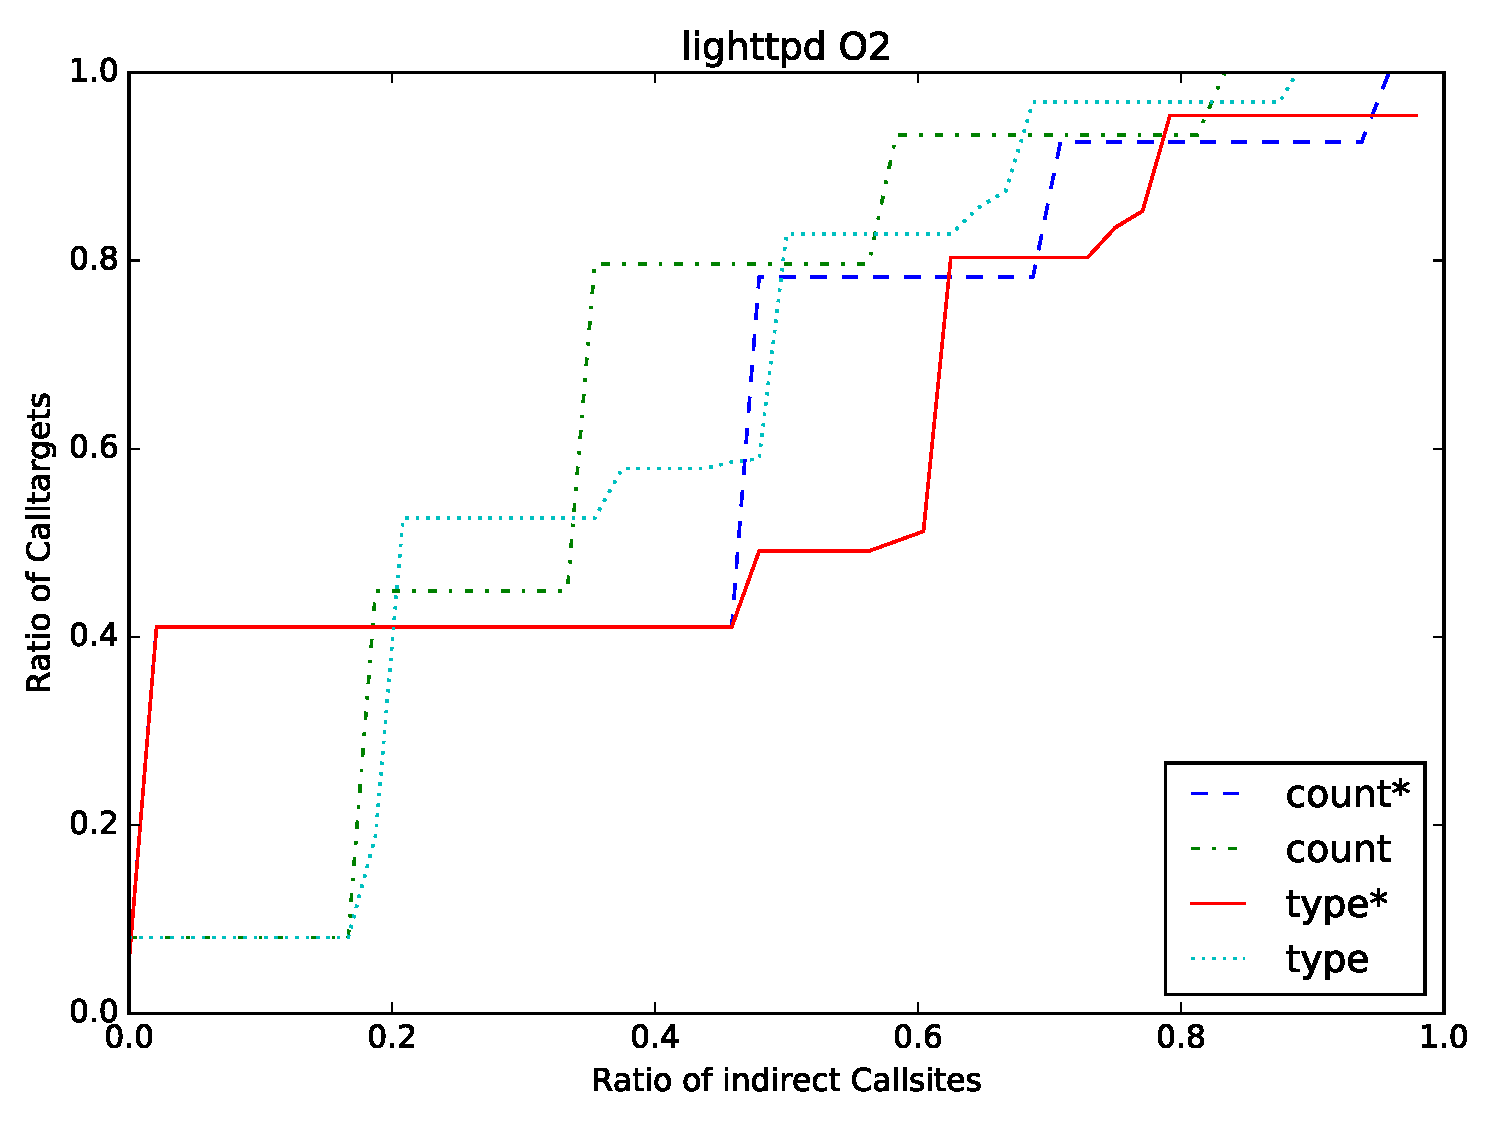
\includegraphics[width=0.5\textwidth]{../MA_Pictures/lighttpd.pdf}\\
%\includegraphics[width=0.5\textwidth]{../MA_Pictures/Memcached.pdf}
%\includegraphics[width=0.5\textwidth]{../MA_Pictures/Mysql.pdf}\\
%\includegraphics[width=0.5\textwidth]{../MA_Pictures/Nginx.pdf}
%\includegraphics[width=0.5\textwidth]{../MA_Pictures/Node.js.pdf}\\
%\includegraphics[width=0.5\textwidth]{../MA_Pictures/Postgresql.pdf}
%\includegraphics[width=0.5\textwidth]{../MA_Pictures/Proftpd.pdf}
%\end{figure}
%

\subsection{Runtime Overhead}
\label{section:typeshieldoverheadperformance}
% \todo[inline]{In this section we need one or two Table similar to what TypeArmor contains, first we need to define the fields which make most sense.}
\begin{figure}[h!]
    \centering
    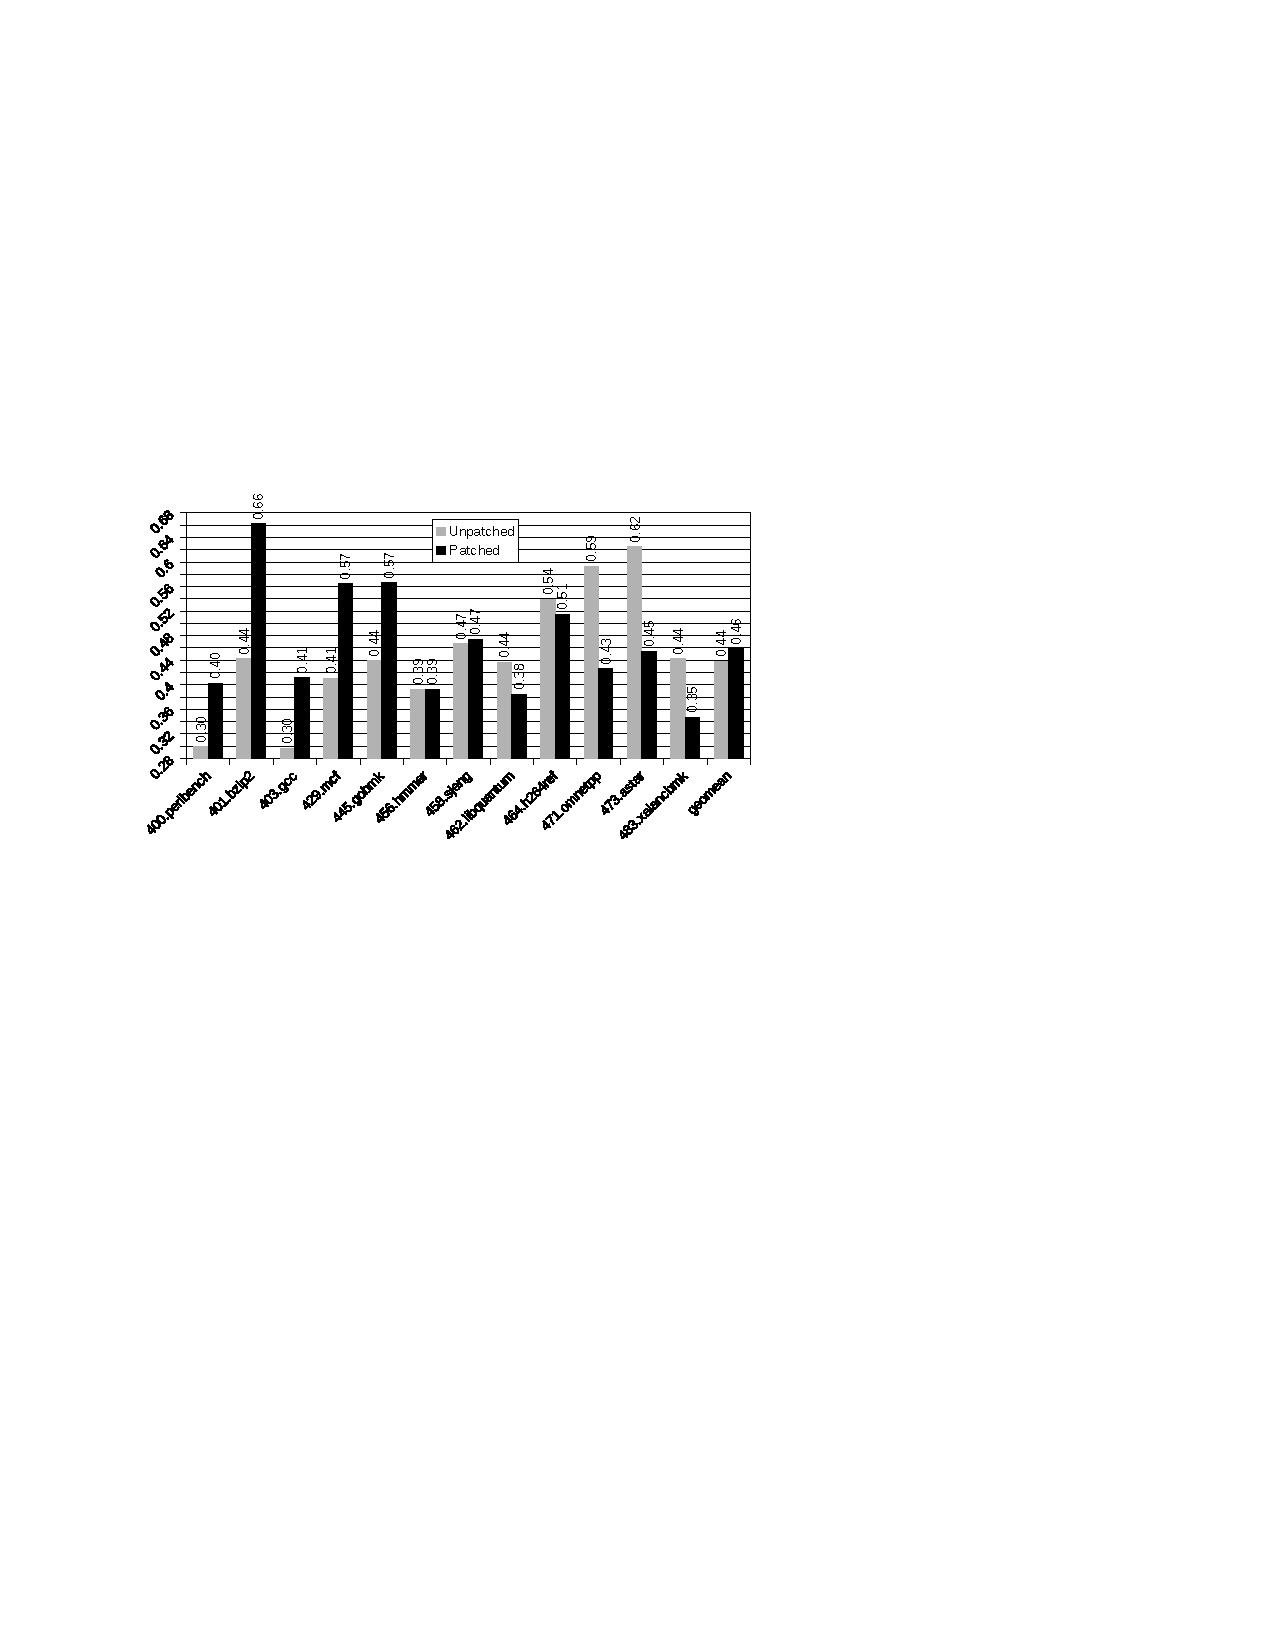
\includegraphics[width=0.47\textwidth]{figures/spec_cpu2006.pdf}
    \caption{SPEC CPU2006 Benchmark Results.
%     \textcolor{red}{TODO-add more description in order to indicate the advantage of our tool. What geomean values are good, low or hig? replace with our values. remove this stub.}
    }
%     \vspace{-.5cm}
    \label{fig:awesome_image}
\end{figure}

Figure~\ref{fig:awesome_image} depicts the runtime overhead obtained by applying our tool to several SPEC CPU2006 benchmarks
in count mode and in count and type mode, respectively.
The obtained geomean runtime overhead is around 4\% performance overhead when instrumenting using DynInst. 
One reason for the performance drop includes cache misses introduced by jumping between the old and the new executable section 
of the binary generated by duplicating and patching. This is necessary, because when
outside of the compiler, it is nearly impossible to relocate indirect control flow. Therefore, 
every time an indirect control flow occurs, one jumps into the old executable section and from 
there back to the new executable section. Moreover, this is also dependent on the actual structure 
of the target, as it depends on the number of indirect control flow operations per time unit.
Another reason for the slightly higher (yer acceptable) performance overhead is due to our
runtime policy which is more complex than that of other state-of-the-art tools.
However, the runtime overhead of \textsc{TypeShield} (4\%) is comparable with other state-of-the-art virtual table defense
tools such as: TypeArmor (3\%), VCI~\cite{vci:asiaccs} (7.79\% overall and 10.49\% on only the SPEC CPU2006 programs), vfGuard~\cite{vfuard:aravind} (10\% - 18.7\%), T-VIP~\cite{gawlik} (0.6\% - 103\%), 
SafeDispatch~\cite{safedispatch:jang} (2\% - 30\%), and VTV/IFCC~\cite{vtv:tice} (8\% - 19.2\%).
Finally, this results qualify \textsc{TypeShield} as a highly practical tool.

\todo[inline]{add a binary patch that does not crash none of the programs from SPEC CPU2006.}
\todo[inline]{need a Table with all the results for each of the SPEC CPU2006 programs and a bar diagram}

\subsection{Instrumentation Overhead}
\label{section:typeshieldoverheadinstrumentation}

\todo[inline]{here we need a bar chart, see TypeArmor paper.}
\todo[inline]{Measure the size (in bytes) of the SPEC2006 testes in RQ3 before and after adding all the patches}

The instrumentation overhead (\textit{i.e.,} binary blow-up) or the change in size due to patching is mostly due to the method DynInst uses to patch binaries. 
Essentially, the executable part of the binary is duplicated and extended with the check we insert. The usual ratio we encountered in our experiments is 
around 40\% to 60\% with Postgres having an increase of 150\% in binary size. One cannot reduce that 
value significantly, because of the nature of code relocation after loosing the information which a compiler has. Especially indirect control flow 
changes are very hard to relocate. Therefore, instead each important basic block in the old code contains a jump instruction to the new position of the basic block.
Finally, this results should not represent an issue for memory resourceful systems on which these applications typically run.

\subsection{Security Analysis}
\label{RQ5: Security Analysis}
% \subsubsection{CDF Analysis}
% \label{CDF Analysis}

\begin{figure}[h] 
\hspace{-.3cm}
  \begin{minipage}[b]{1.0\linewidth}
    \centering
    \resizebox{1.04\columnwidth}{!}{\includesvg{svgs/postgresqlO2}}
%     \vspace{-.7cm}
    \caption{CDF for Postgresql compiled with Clang \texttt{-O2}.} 
    \label{fig7} 
    \vspace{1ex}
  \end{minipage}%%
%   \begin{minipage}[b]{0.5\linewidth}
%     \centering
%     \resizebox{1.04\columnwidth}{!}{\includesvg{svgs/mysqlO2}} 
%     \caption{MySQL.js -O2 CDF.} 
%     \label{fig8} 
%     \vspace{1ex}
%   \end{minipage} 
%   \begin{minipage}[b]{0.5\linewidth}
%     \centering
%     \resizebox{1.04\columnwidth}{!}{\includesvg{proftpdO2.svg}}
%     \caption{Proftpd -O2 CDF.} 
%     \label{fig9} 
%     \vspace{1ex}
%   \end{minipage}%% 
%   \begin{minipage}[b]{0.5\linewidth}
%     \centering
%     \resizebox{1.04\columnwidth}{!}{\includesvg{mysqlO2}} 
%     \caption{Mysql -O2 CDF.} 
%     \label{fig10} 
%     \vspace{1ex}
%   \end{minipage} 
\end{figure}
% Figures~\ref{fig7}, \ref{fig8}, \ref{fig9}, and \ref{fig10} 
Figures~\ref{fig7}
depicts the CDF of the Postgresql program which was compiled with the Clang \texttt{-O2} flag. 
We selected this program randomly from our sample programs. 
The CDFs depict the number of legal callsite targets and the difference between the type and the count policies. 
While the count  policies have only a few changes, the number of changes that can be seen within the 
type policies are vastly higher. The reason for this is fairly straightforward: the number of buckets 
that are used to classify the callsites and calltargets is simply higher. While type policies mostly 
perform better than the count policies, there are still parts within the type plot that are above the 
count plot, the reason for that is also relatively simple: the maximum number of calltargets a 
callsite can access has been reduced. Therefore, a lower number of calltargets is a higher 
percentage than before. However, Figure~\ref{fig7} depicts clearly
that the \textit{count*} and \textit{type*} have higher values as 
\textit{count} and \textit{type}, respectively. This further, confirms our assumptions 
w.r.t. these used metrics. Finally, note that the results dependent on the particular 
internal structure of the hardened programs.

%REMOVED THIS TODO FROM PAPER: todo. Also, add the buckets diagram, see Figure 9 in the typearmor paper.

\subsection{TyperShield Upper Bounds}
\label{RQ6:TyperArmor's Imprecise Parameter-Count Policy}
% \textbf{Permissive Parameter-Count-Based Policies.}
\label{Too Permissive Parameter-Based Policies}
In this section we briefly relate the upper bounds values of \textsc{TypeShield} with the ones of TypeArmor.
TypeArmor~\cite{veen:typearmor} enforces a CFI-based runtime policy in a binary for constraining object dispatches at the callsite based on
function parameter count checks.
We believe that their callsite vs. calltarget set enforcing policy is too permissive and thus
many illegitimate indirect forward edge based control flow transfers are possible. 

Let us consider the following example, where each callsite is
preparing, say, $p=6 \in [1, 6]$ parameters. Then TypeArmor policy would allow calltargets which consume the same number of parameters as
prepared, $c=6 \in [1, 6]$ or a lower value. Thus all possible numerical parameter mismatches are allowed by TypeArmors policy as long
as $p$ is greater or equal than $c$.

% \begin{itemize}
% \item 
TypeArmor \textbf{\textit{ideally}} would allow for a single callsite a set of calltargets containing a maximum of $4096$ possibilities if we 
consider the maximum value of provided parameters to be $p=6$ (due to $p \in [1, 6]$ possible provided parameters). Now, consider 4 C++ integer parameter
types $t$ which use: 8, 16, 32 and 64 byte function parameter register wideness. Thus, we obtain $t^{p}=4^{6}=4096$ allowed calltargets per 
callsite if TypeArmor is used. Note that for simplicity reasons we considered $t=4$ but in practice $t$ is often even larger since there are many types
of parameters in C++. Thus, all these data types are ignored by TypeArmor.

% \item 
TypeArmor \textbf{\textit{actually}} allows more than $t^{p}$ calltargets per callsite. If we have $t=4$ integer types due to TypeArmors overestimation
and underestimation we get for each callsite an additional number of calltargets. Let $p=6$, then we get $c = 6x + 5y+ 4z + 3t + 2p + 1v$ where:
$x$ is the sum of all calltargets consuming 6 parameters, 
$y$ is the sum of all calltargets consuming 5 parameters 
and so on down to 0 parameters. Note that this holds since TypeArmor allows more parameters to be provided than consumed by the calltarget.
Then, $c = 2100 = 600 + 500 + 400 + 300 + 200 + 100 \ iff \ x = y = z = t = p = v = 100$. 
Note that $x = 100$ is feasible number under realistic conditions in large applications (\textit{i.e.,} Google Chrome, Firefox). 
Next $2100$ is added to $4^{6}$. Thus, for a single callsite providing $p=6$ parameters TypeArmor allows theoretically in 
total $4^{6} + 2100 = 6196$ calltargets for each callsite.
Similar reasoning applies to $p=5$ where we get $4^{5} + (1500 = 500 + 400 + 300 + 200 + 100) = \ 1024 + 1500 = 2524 \ iff \ x=y=z=t=p=v=100$ 
allowed calltarget per callsite, or $p \in [1, 4]$, too.
% \end{itemize}

Finally, as it can be observed TypeArmor is too permissive (see also Figure H.1~\cite{vci:asiaccs} for more details), thus 
we present \textsc{TypeShield}, a more precise alternative. \textsc{TypeShield} can deal with the aforementioned 4 types of register widths and can further reduce the the legitimate
calltarget set per callsite as shown herein.

\subsection{Comparison with Shadow-Stack}
\label{Comparison with SafeStack}
There are several tools which provide shadow-stack protection as for example 
the original shadow-stack implementation from Abadi~\cite{abadi:cfi2}(binary-based), SafeStack~\cite{volodymyr:cpi} (compiler based and bypassed~\cite{safestack:bypassing}), 
MoCFI~\cite{mcfi:niu} (compiler based), HAFIX~\cite{hafix} (compiler based and bypassed~\cite{hafix:bypass}), and 
also PathArmor~\cite{veen:cfi} (similarly by-passable as kBouncer, ROPecker, and ROPGuard~\cite{schuster:raid} as it relies on a capacity restricted LBR register.)
which emulates a shadow stack trough validation of the last-branch register (LBR).

There exist many compiler based approaches which can be used to protect backward edges but the only binary
based approach is from Abadi et al.~\cite{abadi:cfi2}. This solution has:
(1) a high rumtime overhead ($\ge$ 21\%), 
(2) is not open source, 
(3) uses a proprietary binary analysis framework (\textit{i.e.,} Vulcan), and
(4) uses a restricted number of labels (\text{i.e.,} each function called from inside another function will get the same label stored in all function shadow stacks, see Figure 1 in~\cite{\textsc{TypeShield}}). 

For this reason we propose an alternative backward edge protection solution which is more effective and is more precise.
In order to show the precision of \textsc{TypeShield} backward edge protection we will give the average wideness between the \textit{max} and 
\textit{min} addresses for all calltarget return sites contained in the MySQL and Node.js programs.

\begin{table}[H]
\centering 
% \resizebox{\columnwidth}{!}{%
 \begin{tabular}{ l | r | r | r | r } 
  \textbf{Program}& \#ct return & \#return addresses    & \# addresses total & \textit{max - min}  \\\hline 
  MySQL           & 192  & 184  & 3   & 1     \\
  Node.js         & 134  & 131  & 1   & 0     \\
  geomean         & 160  & 155  & 1   & 1     \\\hline
\end{tabular}
\caption{Parameter overestimation for ML-G and REC-G.}
\label{Parameter overestimation for ML-G and REC-G.}
% }
\end{table}

Table~\ref{} 

\subsection{Comparison with Other Tools}
\label{RQ5: Is TypeShield better than other tools?}
% \vspace{-.15cm}

\texttt{}

\begin{table}[h]
\resizebox{\columnwidth}{!}{
	\begin{tabular}{l|r|r|r|r|r}%
	\toprule
	\bfseries Target & IFCC  & TypeArmor (CFI+CFC)  & AT  &  TypeShield (count) & TypeShield (type)% specify table head
	\\\midrule
	\csvreader[before filter=\ifthenelse{\equal{\csvcolii}{geomean}}{\csvfilterreject}{\csvfilteraccept},  late after line=\\, late after last line=\\\midrule]{csvs/tools_compare.csv}{
		%1=\target, 2=\opt, 3=\fns, 4=\fnsnotClang, 5=\fnsnotpadyn, 6=\ats, 7=\atnotClang, 8=\atnotpadyn, 9=\cscount, 10=\csClang, 11=\cspadyn
	}
	{\csvcolii & \csvcoliii & \csvcoliv & \csvcolv & \csvcolvi & \csvcolvii}% specify your coloumns here

	\csvreader[before filter=\ifthenelse{\equal{\csvcolii}{geomean}}{\csvfilteraccept}{\csvfilterreject},  late after line=\\, late after last line=\\\bottomrule]{csvs/tools_compare.csv}{
		%1=\target, 2=\opt, 3=\fns, 4=\fnsnotClang, 5=\fnsnotpadyn, 6=\ats, 7=\atnotClang, 8=\atnotpadyn, 9=\cscount, 10=\csClang, 11=\cspadyn
	}
	{\textit{\csvcolii} & \csvcoliii & \csvcoliv & \csvcolv & \csvcolvi & \csvcolvii}% specify your coloumns here
    	\end{tabular}}
%     	}
	\caption {Medians of calltargets per callsite for different tools.
	Note that the smaller the geomean numbers are,
	the better the technique is. AT is a technique which allows calltargets that are address taken. 
	IFCC is a compiler based solution and depicted here as a reference for what is possible when 
	source code is available. TypeArmor and TypeShield on the other hand are binary-based tools. 
	We can observe that our type-based tool reduces the number of calltargets by up to 35\% when 
	compared to the AT method and by 13\% on average when comparing with TypeArmor.}
% 	Note that we removed Nginx out of the table
% 	because at the time of our evaluation it produced outlier results which we further wanted to investigate.
% 	Thus, increasing even more the offered security benefit.} 
	\label{tbl:toolcompare}
% 	\vspace{-.5cm}
\end{table}

Table~\ref{tbl:toolcompare} depicts 
a comparison between \textsc{TypeShield}, TypeArmor and IFCC with respect to the count of calltargets per callsites. 
The values depicted in this table for TypeArmor and IFCC are taken from the original TypeArmor paper.
We compare our version of address taken analysis (AT), TypeArmor, \textsc{TypeShield} (count), \textsc{TypeShield} (type) and IFCC. The first 
thing to notice is that when comparing these values, one can see that we did not depicted a separation based on return type or the 
CFC that TypeArmor introduced. Therefore, when implementing those measures, we think that our solution would improve even 
more with respect to precision than TypeArmor. While we anticipate that it is possible to surpass TypeArmor implementing those two solutions 
in our tool, we deem it very hard to compete with IFCC, which can directly operate on the source code level 
and has access to more possibilities than simply inspecting function parameters or return values.
Nevertheless, \textsc{TypeShield} represents a strong improvement w.r.t. calltarget per callsite reduction in binary programs.

\subsection{Effectiveness Against COOP}
\label{Effectiveness Against COOP}
We investigated the effectiveness of \textsc{TypeShield} against the COOP
attack by looking at the number of register arguments which can be used to enable 
data-flow between gadgets. In order to determine how many arguments 
remain unprotected after we apply the forward edge policy of \textsc{TypeShield}
we compared the number of parameter overestimation and compare it with the ground truth
obtained with the help of an LLVM compiler pass. Next we used some heuristics to determine 
how many ML-G and REC-G callsites exist for each of the C++ only server applications.
Finally, we compared these results with the one obtained by TypeArmor.

\begin{table}[H]
\centering 
% \resizebox{\columnwidth}{!}{%
 \begin{tabular}{ l | r | r | r | r | r | r | r } 
                         \multicolumn{8}{c}{\hspace{3cm}\textbf{Overestimation}} \\
  \textbf{Program}& \#cs & 0    & +1  & +2  & +3  & +4  & +5  \\\hline 
  MySQL (ML-G)    & 192  & 184  & 3   & 1   & 0   & 1   & 3   \\
  Node.js (ML-G)  & 134  & 131  & 1   & 0   & 1   & 0   & 1   \\
  geomean         & 160  & 155  & 1   & 1   & 1   & 1   & 1   \\\hline
  MySql (REC-G)   & 289  & 273  & 10  & 2   & 3   & 0   & 1   \\
  Node.js (REC-G) & 72   & 69   & 2   & 0   & 0   & 0   & 1   \\
  geomean         & 144  & 137  & 4   & 1   & 1   & 1   & 1   \\\hline
\end{tabular}
\caption{Parameter overestimation for ML-G and REC-G.}
\label{Parameter overestimation for ML-G and REC-G.}
% }
\end{table}
Table~\ref{Parameter overestimation for ML-G and REC-G.} depicts the results obtained
after counting the number of perfectly and overestimation of protected ML-G and 
REC-G gadgets. As it can be observed we obtained a
96\% (184 vs. 192) accuracy (geomean) of perfectly protected ML-G callsites for MySQL while
TypeArmor obtaines for the same program an 94\% accuracy (geomean). Further,
\textsc{TypeShield} obtained a 97\% (131 vs. 134) accuracy (geomean) for Node.js while TypeArmor
obtained 95\% accuracy on the same program.
Further, for the REC-G case \textsc{TypeShield} obtained an
94\% (273 vs.289) exact argument accuracy for MySQL while TypeArmor had 86\%.
For Node.js \textsc{TypeShield} obtained an exact parameter 
matching of 95\% (69 vs. 72) while TypeArmor obtained an 96\% perfect matching.

Overall \textsc{TypeShield}s forward edge policy obtained an perfect accuracy 
of 95\% while TypeArmor obtained 92\%. While this is not a big difference
we point out that the remaining overestimated parameters represent 5\% and this 
do not leave much room for the attacker to perform her attack.


\subsection{Mitigation of Advanced Code-Reuse Attacks}
\label{Mitigation of Advanced Code-Reuse Attacks}

\begin{table}[H]
\centering 
% \resizebox{\columnwidth}{!}{%
 \begin{tabular}{ l  r  r  } 
  \textbf{Exploit}& Stopped & Remark  \\\hline 
  COOP ML-G       &         &         \\
  IE 32 bit       &         &         \\
  IE 1 64-bit     &         &         \\
  IE 2 64-bit     &         &         \\
  Firefox         &         &         \\\hline
  COOP ML-REC     &         &         \\
  Chrome          &         &         \\\hline
  Control Jujutsu &         &         \\
  Apache          &         &         \\
  Nginx           &         &         \\\hline
  Other Backward edge          &         &         \\
  
\end{tabular}
\caption{Parameter overestimation for ML-G and REC-G.}
\label{Parameter overestimation for ML-G and REC-G.}
% }
\end{table}
